\documentclass[a4paper,11pt]{article}
\usepackage{latexsym}
\usepackage[american]{babel}
\usepackage{lmodern}
\usepackage[utf8]{inputenc}
\usepackage[T1]{fontenc}
\usepackage{longtable}
%\usepackage[dvips]{graphicx}
\usepackage{graphicx}

%\usepackage[pdftex]{hyperref}
\usepackage{hyperref}
\usepackage{amsmath}  % for equation environment
\usepackage{enumitem} % nolistsep to reduce list spacing

%\usepackage{lscape}
%\usepackage{pdflscape}
\usepackage{setspace}

% Reference https://www.physicsforums.com/threads/line-spacing-in-latex.534380/


\newcommand\ddfrac[2]{\frac{\displaystyle #1}{\displaystyle #2}}

% define the title
\author{Hilton Fernandes}
\title{Simulation test scenarios -- TB}
% \date{}	

\frenchspacing

\pagestyle{myheadings}

\markboth{Simulation test scenarios -- TB}
         {Simulation test scenarios -- TB}

\addtolength{\hoffset}{-1,5cm}
\addtolength{\textwidth}{+2.3cm}

\addtolength{\voffset}{-1,2cm}
\addtolength{\marginparwidth}{-0,5cm}
\addtolength{\textheight}{+3.5cm}
\addtolength{\textwidth}{+1.2cm}

% \linespread{1.5}

\begin{document}

% generates the title
\maketitle

% insert the table of contents
\tableofcontents

\pagebreak

\section{Procedures}

\subsection{To buy an ask order {\tt BUY}}

Provided that the asked price $r_A$ is lower than $r_S$, the price registered in the 
source wallet $w_S$, the {\tt BUY} procedure has five steps:
\begin{enumerate}
    \item \label{itm:BUY-1} {\tt BUY\_1}: 
	the balance in $w_S$ is converted to source coin: $b_S \times r_S$;
	
    \item \label{itm:BUY-2} {\tt BUY\_2}: 
	That balance is then converted to target, according to the asked rate 
	\begin{equation*}
	    \frac{b_S \times r_S}{r_A}; 
	\end{equation*}
	
    \item \label{itm:BUY-3} {\tt BUY\_3}: 
	the purchase, or the amount to be bought, is the minimum among what can is in 
	the wallet and what is being sold:
	\begin{equation*}
	    p_T = min \left( \frac{b_S \times r_S}{r_A}, a_T \right); 
	\end{equation*}
	
    \item \label{itm:BUY-4} {\tt BUY\_4}:
	the purchased amount is subtracted from the balance in the source wallet $w_S$:
	\begin{equation*}
	    a'_S = a_S - p_T \frac{r_A}{r_S};
	\end{equation*}
	The ratio $r_A / r_S$ takes into account that the source coin in the $w_S$ corresponds
	to a higher valued target coin.
	
    \item \label{itm:BUY-5} {\tt BUY\_5}:
	the purchased amount is added to the balance in the target wallet $w_T$:
	\begin{equation*}
	    a'_T = a_T + P_T.
	\end{equation*}
	
\end{enumerate}

{\em OBS:} In a real exchange situation, the $p_T$ amount is reserved in the source wallet and is 
only added to the target wallet when a real sale happens: there can be a situation when oner or 
more faster buyers get all the ask offer, or part of it. In that case, the reserved amount (or 
part of it) can be returned to the normal operation of the source wallet.

\subsection{To sell for a bid order {\tt SELL}}

Provided that the asked price $r_B$ is higher than $r_T$, the price registered in the 
target wallet $w_T$, the {\tt SELL} procedure has three steps:

\begin{itemize}
    \item \label{itm:SELL-1} {\tt SELL\_1}: 
	the transfer value, or the amount to be sold, is the minimum among what can is in 
	the target wallet and what the bid offer wants to buy:
	\begin{equation*}
	    t_T = min (a_T, b_T); 
	\end{equation*}
	
    \item \label{itm:SELL-2} {\tt SELL\_2}:
	the transfer amount is subtracted from the balance in the target wallet $w_T$:
	\begin{equation*}
	    a'_T = a_T - t_T;
	\end{equation*}
	
    \item \label{itm:SELL-3} {\tt SELL\_3}:
	the purchased amount is added to the balance in the source wallet $w_S$:
	\begin{equation*}
 	    a'_S = a_S + t_T.
	\end{equation*}
	
\end{itemize}
{\em OBS:} In a real exchange situation, the $t_T$ amount is reserved in the target wallet and is 
only added to the source wallet when a real sale happens: there can be a situation when one or 
more faster sellers get all the bid offer, or part of it. In that case, the reserved amount (or 
part of it) can be returned to the normal operation of the source wallet.

\section{Simple 1: everything constant}
\label{sec:Simple1}

\begin{figure}[!hbpt]
  \centering
  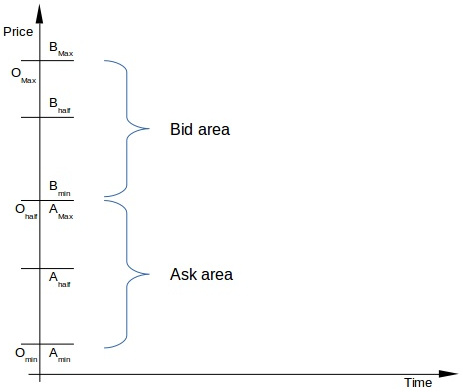
\includegraphics[scale=0.5]{Simple1}
  \caption{Graphical description of scenario {\em Simple1}}
  \label{fig:Simple1}
\end{figure}    

\subsection{Conditions}
\begin{itemize}
    \item All orders in the range $[ O_{min}, O_{Max}]$;
    \item Middle order at $O_{half} = (O_{min} + O_{Max}) / 2$;
    \item All orders have amount $a$;
    \item Ask orders belong to $[ A_{min}, A_{Max}]$, where 
        $A_{min} = O_{min}$, and $A_{Max} = O_{half}$. 

        In this scenario, all ask orders have price 
        $r_A = A_{half} = (A_{min} + A_{Max}) / 2$.
    \item Bid orders belong to $[ B_{min}, B_{Max}]$, where 
        $B_{min} = O_{half}$, and $B_{Max} = O_{Max}$. 

        In this scenario, all bid orders have price 
        $r_B = B_{half} = (B_{min} + B_{Max}) / 2$.
    \item There is a wallet for target coin, and and another for source coin. 
	
	Both wallets are considered in terms of the target coin, even though the source coin
	wallet in reality has source coin values. That eases the calculations, and is in line with 
	the common practice in the exchanges, where ask and bid orders are given in terms of the 
	target coin only.
	
	The values in the source coin are associated with a conversion rate for the target coin, 
	what permits that;
	
    \item The wallet for {\em target} coin $w_T$ has an initial amount $a_t = a$, and 
        a constant rate 
        \begin{equation*}
	    r_T = A_{half}= r_A; 
        \end{equation*}
        
    \item The wallet for {\em source} coin $w_S$ has an initial amount $a_S = a$, and 
        a constant rate
        \begin{equation*}
	    r_S = B_{half} = r_B; 
        \end{equation*}

    \item The simulation starts with an ask order;
    \item It is succeeded by a bid order, and then by an ask order -- and so
	on indefinitely: an ask then a bid, then an 
ask\ldots{}
\end{itemize}

\subsection{Alternative \ref{sec:Simple1}.1 -- 1st Ask}

Here follow the orders:

\subsubsection{Ask order \# 1} 

When the 1st {\bf ask} order arrives with rate $A_{half}$, and an amount $a$, the {\em source} 
wallet has an amount $a$, and a buy price of $r_S = B_{half}$. Since the buy rate $r_S$ is above the 
ask rate $A_{half}$, the target coin will be bought.
	
\begin{itemize}
    \item  In the {\tt BUY\_1} (step \ref{itm:BUY-1}): the balance is converted to 
	source coin: $b_S \times r_S = a \times r_S$;
		
    \item Following the {\tt BUY\_2} step (item \ref{itm:BUY-2}): the balance in 
	source coin is converted to target coin using the $r_A$ rate:
	\begin{equation*}
	    \frac{a \times r_S}{r_A} = a \frac{r_S}{r_A}
	\end{equation*}
			
    \item Following step {\tt BUY\_3} (item \ref{itm:BUY-3}):
	Since $r_S > r_A$, the expression from {\tt BUY\_1} is larger than $a$, the amount
	in the ask order. So, the value to be bought is simply $a$; 
	
    \item Following step {\tt BUY\_4} (item \ref{itm:BUY-4}): Since $a$ was used, it is
	subtracted from the previous balance in the wallet $w_S$:
	\begin{equation*}
	    a \frac{r_S}{r_A} - a = a \left( \frac{r_S}{r_A} - \frac{r_A}{r_A} \right) 
		                  = a \frac{r_S - r_A}{r_A}.
	\end{equation*}
		
    \item Following step {\tt BUY\_5} (item \ref{itm:BUY-5}):
	the purchased amount $a$ is added to the balance in the target wallet $w_T$. Since
	it was $a$ it becomes
	\begin{equation*}
	    a'_T = a_T + P_T = a + a = 2a.
	\end{equation*}
		
    \end{itemize}
	
        
\subsubsection{Bid order \# 1} 
    
Now comes a {\bf bid} order that wants to buy an amount $a$ of {\bf target} coin, at a rate 
$B_{half}$.  Since the sale rate $r_T = A_{half}$ is below the bid rate, the target coin will be 
sold. That is: the target will be sold by a price higher than it was bought.
	
\begin{itemize}
    \item  In the {\tt SELL\_1} (step \ref{itm:SELL-1}): The bid offers will buy $a$ target coins.
	The target coin has $2a$ -- so the minimum is $a$;
	
    \item Following the step {\tt SELL\_2} (step \ref{itm:SELL-2}), the minimum computed in the 
	previous item will be subtracted from the target wallet $w_s$: 
	\begin{equation*}
	    a'_T = 2a - a = a.
	\end{equation*}
	
    \item according to {\tt SELL\_3} (item \ref{itm:SELL-3}):
	the amount transfered from the sale is added to the balance in the source wallet $w_S$:
	\doublespacing
	\begin{equation*}
	\begin{array}{lcl}
 	    a'_S = a_S + t_T & = & a \ddfrac{r_S - r_A}{r_A} + a \\
 	                     & = & a \ddfrac{r_S - r_A}{r_A} + a \ddfrac{r_A}{r_A} \\
 	                     & = & a \left( \ddfrac{r_S - r_A + r_A}{r_A} \right) \\
 	                     & = & a \ddfrac{r_S}{r_A} \\
 	                     & = & a \ddfrac{r_B}{r_A}.
	\end{array}
	\end{equation*}
	\singlespacing
	
	Since $r_S = r_B > r_A$, the balance in the source wallet is larger than $a$.

\end{itemize}

	
\subsubsection{Ask order \# 2}
    
Then comes another {\bf ask} order, and it has price $A_{half}$, and an amount $a$. Since the buy price 
$r_S = B_{half}$ is higher than $A_{half}$, the target coin will be bought.
	
\begin{itemize}
    \item Following step {\tt BUY\_1} (item \ref{itm:BUY-1}): 
	converting the balance $w_S$ to source coin: 
	\begin{equation*}
	    a \ddfrac{r_B}{r_A} \times r_S = \ddfrac{r_B^2}{r_A},
	\end{equation*}
	since $r_S = r_B$;
  
    \item Following step {\tt BUY\_2} (item \ref{itm:BUY-2}): 
	\begin{equation*}
	    a \ddfrac{r_B}{r_A} \times \ddfrac{1}{r_A} = a \ddfrac{r_B^2}{r_A^2};
	\end{equation*}
	  
    \item Following step {\tt BUY\_3} (item \ref{itm:BUY-3}): 
	since $\ddfrac{r_B^2}{r_A^2} > 1$, the minimum between the amount in the ask offer and 
	what is in the source wallet $w_S$ is $a$;
	
    \item Following step {\tt BUY\_4} (item \ref{itm:BUY-4}): 
	\begin{equation*}
	    a'_{S} = a \ddfrac{r_B^2}{r_A^2} - a = a \ddfrac{r_B^2 - r_A^2}{r_A^2}.
	\end{equation*}
	
    \item Following step {\tt BUY\_5} (item \ref{itm:BUY-5}): 
	\begin{equation*}
	    a'_{T} = a + a = 2 a.
	\end{equation*}
   
\end{itemize}
	
\subsubsection{Bid order \# 2} 
    
Now comes a {\bf bid} order that wants to buy an amount $a$ of {\bf target} coin, at a rate 
$r_B = B_{half}$.  Since the sale rate $r_T = A_{half}$ is below the bid rate, the target coin will be 
sold. That is: the target will be sold by a price higher than it was bought.

------------------------------------------------------------------------------------------------------

\begin{itemize}
    \item  In the {\tt SELL\_1} (step \ref{itm:SELL-1}):
    	
    \item Following the step {\tt SELL\_2} (step \ref{itm:SELL-2}), 
	
    \item according to {\tt SELL\_3} (item \ref{itm:SELL-3}):

\end{itemize}

	
\subsubsection{Ask order \# 3} 
	
\subsubsection{Bid order \# 3} 
	
\subsubsection{Ask order \# 4}
	
\subsubsection{Bid order \# 4}
	
\subsubsection{Ask order \# 5} 
	
\subsubsection{Bid order \# 5} 
	
\subsubsection{History of wallet balances} 

\subsection{Alternative \ref{sec:Simple1}.2 -- 1st Bid}

\begin{table}[!hbpt]
    \centering
    \begin{tabular}{r|l|l|l}
	\hline
	{\bf Step \#} & {\bf Order} & \multicolumn{2}{|l} {\bf Balance} \\
	              &             & {\bf Source coin} & {\bf Target coin} \\
	\hline
	            0 & Start      &  $a$               & $a$ \\
	\hline
	            1 & Ask \# 1   &                    & \\
	\hline
	            2 & Bid \# 1   &                    & \\
	\hline
	            3 & Ask \# 2   &                    & \\
	\hline
	            4 & Bid \# 2   &                    & \\
	\hline
	            5 & Ask \# 3   &                    & \\
	\hline
	            6 & Bid \# 3   &                    & \\
	\hline
	            7 & Ask \# 4   &                    & \\
	\hline
	            8 & Bid \# 4   &                    & \\
	\hline
	            9 & Ask \# 5   &                    & \\
	\hline
	           10 & Bid \# 5   &                    & \\
	\hline
    \end{tabular}
    \caption{}

\end{table}



\section{Simple 2: Simple 1 \& relaxing order amount}
\section{Simple 3: Simple 2 \& relaxing order sequence}
\section{Simple 4: what next ?}

\end{document}
